\chapter{Recupero e Utilizzo delle Point Cloud}
\label{cap:ReceUsoPCL}

In questo capitolo si descriverà come è stato scritto un servizio di retrival delle pointcloud a partire dalle mappe e di come queste vengano poi utilizzate.

	\section{ROS (Robotic Operating System)}
	\label{sez:ROS}
ROS è un framework flessibile open source che nasce per lo sviluppo e la programmazione dei robot ed è infatti molto utilizzato nell'ambito della robotica di servizio. Il software è liberamente disponibile dal sito ufficiale\cite{ROS}.
Le peculiarità del framework sono simili a quelle di un qualsiasi sistema operativo:
\begin{enumerate}
 \item Capacità di fornire astrazione dell’hardware.
 \item Modularità (cioè la possibilità di avere diverse parti del sistema che lavorano autonomamente al fine di raggiungere un obiettivo comune).
 \item Possibilità di controllare i dispositivi tramite driver. 
 \item Possibilità di gestione delle applicazioni (package).
\end{enumerate}

ROS è costituito fondamentalmente da una rete di processi che vengono eseguiti in parallelo e che comunicano tra di loro sfruttando un architettura Peer-to-Peer.
Essi vengono comunemente chiamati \textit{Nodi} e costituiscono uno degli elementi principali del sistema.
Per essere eseguiti è necessario, innanzitutto, avviare un server principale tramite comando \textit{roscore}. Denominato ROS Master (o Core) consente di effettuare operazioni di routing permettendo ai processi di comunicare tra loro.\\
Nella comunicazione, i \textit{Nodi} si scambiano \textit{messaggi}. ROS fornisce una grande quantità di messaggi predefiniti ma è ovviamente possibile crearne di nuovi a seconda delle proprie esigenze.
Sostanzialmente un nodo è un programma che si interfaccia con il ROS Master per comunicare con altri nodi tramite messaggi.
Il sistema di scambio di messaggi è molto simile all’architettura pub/sub: esistono nodi \textit{talker} (Publisher) e nodi \textit{listener} (Subscriber).\\ 
Per circolare i messaggi possono sfruttare \textit{topic} o \textit{servizi}:
\begin{itemize}
\item \textbf{Topic}: i nodi Publisher creano il Topic (canale di comunicazione) e su di esso pubblicano i messaggi, mentre i nodi Subscriber vi si sottoscrivono per poterne ricevere il contenuto. 
Più nodi possono sottoscriversi allo stesso topic e ogni nodo può pubblicare su uno o più topic contemporaneamente.
\begin{figure}[h!]
    \centering
    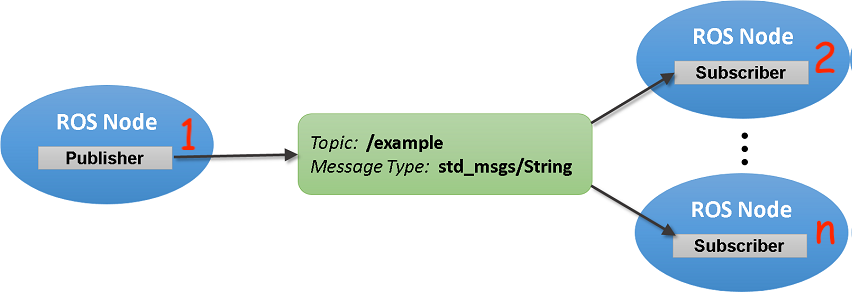
\includegraphics[scale=0.25]{Immagini/topic.png}
    \caption{schema di comunicazione \textit{Publisher-Subscriber} tramite topic}  
    \label{fig:topic}
\end{figure}

\item \textbf{Servizi}: forniscono la possibilità di creare una comunicazione sincrona tra un nodo client, che può richiedere un servizio mandando una \textit{request} ed un nodo server, che riceverà la richiesta e risponderà con una \textit{response}. 
\begin{figure}[h!]
    \centering
    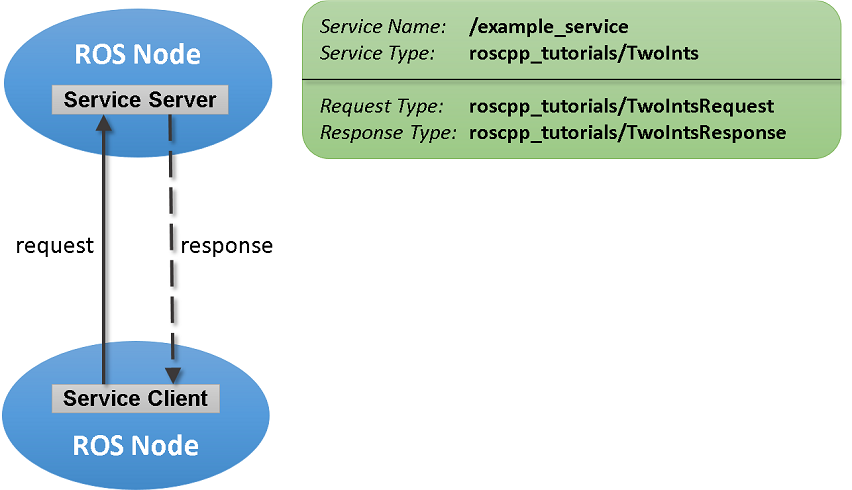
\includegraphics[scale=0.25]{Immagini/servizi.png}
    \caption{schema di comunicazione \textit{Client-Server} tramite servizio}  
    \label{fig:service}
\end{figure}
\end{itemize}

ROS in particolare nella versione Kinetic basata sulla versione 16.04 di ubuntu è alla base di RLE su cui si è andato a lavorare.

\section{RLE (Road Layout Estimation)}
\label{sez:RLE}

\textit{Road Layout Estimation}\cite{Ballardini2015} è un framework probabilistico per l'interpretazione di scene in contesto urbano. Gli elementi da interpretare in una scena urbana possono essere sia di natura \textit{statica}, come edifici, cartelli stradali o incroci, sia di natura \textit{dinamica}, come altri veicoli o persone.

Il framework è modulare e consente la localizzazione attraverso diverse fonti di date. I dati possono provenire da sensori fisici come camere, LiDAR e GPS, o da sensori virtuali ovvero moduli software che analizzano la scena e ne estraggono diverse caratteristiche.

A differenza dei framework già esistenti che prevedono un insieme finito di sensori definito a priori durante la fase di design, \textit{RLE} si basa sull'assunzione che diverse informazioni da diverse fonti possono essere disponibili a frequenze diverse, assenti per un certo periodo, o addirittura utili solo in specifiche situazioni. 

\subsection{Architettura}

L'approccio con cui \textit{RLE} localizza il veicolo nella mappa si basa su un filtro definito particle filtering\cite{thrun2005probabilistic}, la scena viene destcritta attraverso delle \textit{layout hypothesis}(LH). Le LH sono un insieme di elementi che descrivono lo stato del veicolo. In particolare danno informazioni riguardo:

\begin{itemize}

\item Lo \textit{stato} vero e proprio del veicolo, espresso tramite pose e velocità in \textit{6DoF}.

\item Il vettore di \textit{Layout Component}, o LC, ovvero i modelli geometrici o semantici associati agli elementi della scena.

\item lo \textit{score} del layout, ovvero una stima della verosimiglianza dell'ipotesi

\item Il \textit{modello di movimento}, che descrive come l'ipotesi evolve nel tempo.

\end{itemize}

I \textit{layout component}(LC) sono alla base del processo di interpretazione della scena, ogni istanza di LC vive indipendentemente dalle altre, sia che appartengano alla stessa ipotesi o meno, per questo nell'implementazione di ognuna sono definite le funzioni che calcolano sia lo score che la propagazione del moto.

Ogni LC viene creato nel momento in cui \`e riconosciuto da uno specifico detector, che comunica poi al \textit{Layout Manager} i dati di interesse. Il \textit{Layout Manager} \`e il nodo principale del sistema, e il suo compito \`e quello di gestire tutte le diverse ipotesi di struttura della scena nel tempo. Per fare questo assegna a ciascuna ipotesi un punteggio su quanto essa risulti essere verosimile. Di seguito è possibile vedere lo schema ad alto livello di funzionamento del framework.

\begin{figure}[h!]
    \centering
    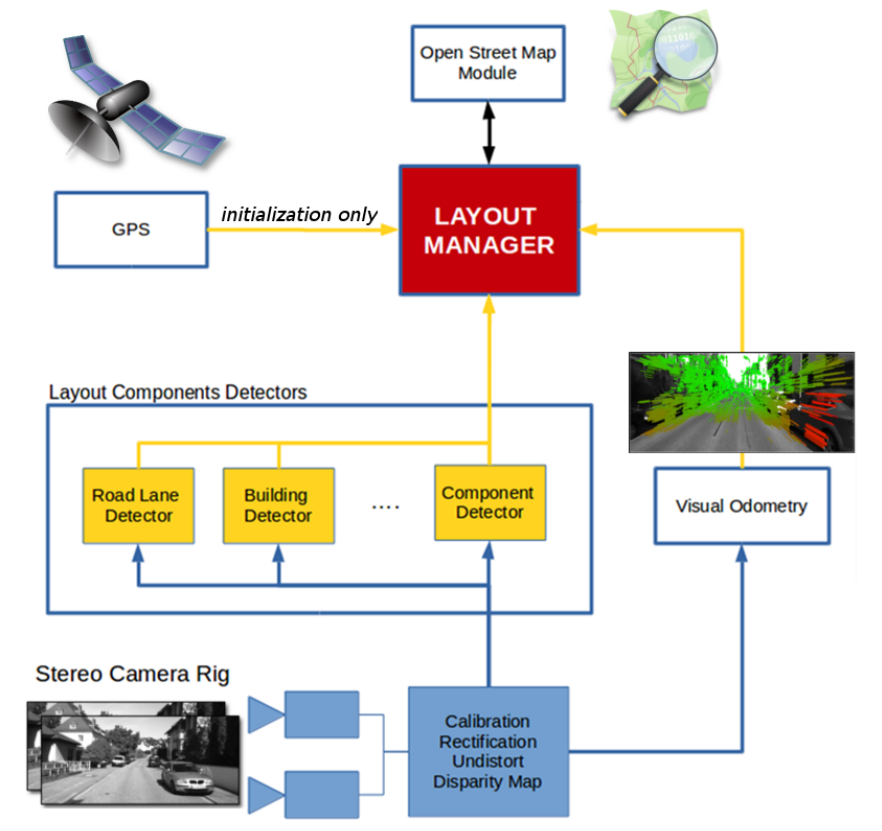
\includegraphics[width=0.8\textwidth]{Immagini/rle.png}
    \caption{Schema ad alto livello del funzionamendo di RLE}
    \label{fig:rle}
\end{figure}

Nel lavoro ci si è concentrati sull'estensione di IRA OpenStreetMaps e di IRA Building Detector\cite{CattaneoSergioTesi} per permettere il recupero e l' utilizzo delle point cloud salvate all'interno delle mappe.

\section{IRA OpenStreetMap}
\label{sez:IRAOSM}
IRA OpenStreetMap è un componente di RLE che consente di caricare le mappe per poi utilizzarle successivamente durante la navigazione, esso è un fork di \href{https://github.com/ros-geographic-info/open_street_map}{ROS Open\_steet\_map} con alcune sostanziali modifiche per il suo utilizzo all'interno di RLE.

Esso è stato modificato in un suo nodo che si occupa dell' acquisizione della mappa. Ad esso sono state fatte delle modifiche riguardanti:
\begin{enumerate}
    \item La selezione della sorgente da cui scaricare la mappa.
    \item La possibilità di scaricare solo gli edifici con una point cloud associata.
\end{enumerate}{}

Per quanto riguarda la prima parte il nodo preesistente consentiva il download soltanto dall'API Overpass globale è stato per tanto necessario inserire la possibilità di utilizzare l'API locale che è stata descritta nel capitolo precedente.\\
Si è quindi aggiunto un argomento booleano \textit{local} al nodo che consente di selezionare su quale server andare ad effettuare la query:

\begin{lstlisting}[caption={Aggiunta del parametro per il download dal server in locale},captionpos=b,language=cpp]
#Aggiunta di un nuovo parametro booleano
TCLAP::SwitchArg localArg("l","local","use local server", cmd, false);
bool local = localArg.getValue();
\end{lstlisting}

Si è poi andato ad introdurre un selettore per selezionare l'url da utilizzare.

\begin{lstlisting}[caption={Selezione del server da utilizzare per la query},captionpos=b,language=cpp]
 if (local){
            osm_api_url = "http://gas2008-server.disco.unimib.it:5001/api/interpreter?data=(" + highwaysQuery + buildingQuery + paramQuery + ");(._;>;);out%20meta;";
        } else {
            osm_api_url = "http://www.overpass-api.de/api/interpreter?data=(" + highwaysQuery + buildingQuery + paramQuery + ");(._;>;);out%20meta;";
        }
\end{lstlisting}

Il secondo punto invece implicava l'inserimento di un nuovo parametro per la scelta di scaricare tutti gli edifici o solamente gli edifici che avevano una point cloud associata. Esso è risultato nell'implementazione all'interno del nodo della query di Overpass API descritta precedentemente \ref{lst:OSMQuery}, aggiunta in modo molto semplice, dopo aver definito il nuovo parametro booleano \textit{buildingPCL} in modo analogo a sopra, con il seguente frammento di codice:

\begin{lstlisting}[caption={Inserimento della query con cui scaricare gli edifici con la PCL associata.},captionpos=b,language=cpp]
if (buildingPCL)
        {
            buildingQuery = "node[building:facade:pcl]" + area + ";"
            + "way[building:facade:pcl]" + area + ";"
            + "relation[building:facade:pcl]" + area + ";";
        }
\end{lstlisting}

E' stato poi necessario implementare un \textit{service} ROS che andasse a recuperare le point cloud ottenute dagli edifici, esso si comporta in modo similare al \textit{service getNearBuildings} già esistente dentro IRA OpenStreetMap  che invece di restituire un messaggio di tipo 
\textit{geometry\_msgs/Point} ovvero una lista di punti restituisse un messaggio di tipo \textit{sensor\_msgs/PointCloud2} ovvero la point cloud che descrive la facciata richiesta in quel momento.\\

Il servizio, denominato \textit{getNearestBuildingFacade}, è definito come segue:

\begin{lstlisting}[caption={Definizione del servizio per il retrival delle facciate},captionpos=b,language=cpp]
#request fields (float64 = C++ double)
float64 latitude
float64 longitude
float64 theta
float64 radius
---
#response fields (float64 = C++ double)
sensor_msgs/PointCloud2 facadecloud
\end{lstlisting}

Il servizio prende in output latitutine, longitudine correnti e i raggi a cui ricercare gli edifici e ritorna la point cloud dell'edificio più vicino, il funzionamento è il seguente:

\subsection{Recupero delle way}
\begin{lstlisting}[caption={Recupero delle way con il tag inerente alla facciata.},captionpos=b,language=cpp]
 Xy center = latlon2xy_helper(req.latitude, req.longitude);
    vector<shared_ptr<Osmium::OSM::Way const> > way_vector;
    for(std::set<shared_ptr<Osmium::OSM::Way const> >::iterator way_itr = oh.m_ways.begin(); way_itr != oh.m_ways.end(); way_itr++
    {
        const char* building_tag = (*way_itr)->tags().get_value_by_key("building:facade:pcl");
        if (!building_tag)
            continue;
        Osmium::OSM::WayNodeList waylist = (*way_itr)->nodes();
        for(Osmium::OSM::WayNodeList::iterator node_list_itr = waylist.begin(); node_list_itr != waylist.end(); node_list_itr++ )
        {
            double lat = node_list_itr->position().lat();
            double lon = node_list_itr->position().lon();
            Xy way_node_xy = latlon2xy_helper(lat, lon);
            double distance = get_distance_helper(center.x, center.y, way_node_xy.x, way_node_xy.y);
            if(distance <= req.radius)
            {
                way_vector.push_back(*way_itr);
                break;
            }
       }
    }
    if(way_vector.size() == 0){
        ROS_ERROR_STREAM("     No map nodes found next to particle. Distance radius: " << req.radius << " m");
        return false;
    }
\end{lstlisting}{}

Questa prima parte è molto similare al servizio già esistente, essa consente di andare a trovare e salvare tutte le way in un raggio ben definito rispetto alla posizione corrente, la differenza rispetto al servizio per il recupero dei generici edifici è che si va a filtrare non solo sul tag \textit{building} che indica se la way è un edificio o meno ma si utilizza il più specifico tag \textit{building:facades:pcl} che indica se un edificio ha una point cloud associata o meno.
\newpage
\subsection{Recupero delle point cloud}
\begin{lstlisting}[caption = {Recupero e download delle pointcloud},numbers=left,captionpos=b, language = cpp]
 for(vector<shared_ptr<Osmium::OSM::Way const> >::iterator way_itr = way_vector.begin(); way_itr != way_vector.end(); way_itr++)
    {
        Osmium::OSM::WayNodeList way_n_list = (*way_itr)->nodes();
        for(Osmium::OSM::WayNodeList::iterator node_list_itr = way_n_list.begin(); node_list_itr != way_n_list.end() - 1; node_list_itr++ )
        {
        const char* facadepclurl = obj.tags().get_value_by_key("building:facade:pcl");
        if (facadepclurl) {
            resource_retriever::Retriever r;
            resource_retriever::MemoryResource resource;
                try
                {    
                    resource = r.get(facadepclurl); 
                }
                catch (resource_retriever::Exception& e)
                {
                    ROS_ERROR("Failed to retrieve file: %s", e.what());
                }
                FILE* f = fopen("cloud.pcd", "w");
                fwrite(resource.data.get(), resource.size, 1, f);
                fclose(f);
                
                sensor_msgs::PointCloud2 output;
                pcl::PointCloud<pcl::PointXYZ> cloud;
                pcl::io::loadPCDFile ("cloud.pcd", cloud);
                pcl::toROSMsg(cloud, output);
                resp.facadecloud = output;
            }
        }
    }
\end{lstlisting}{}

La seconda parte, che si occupa del recupero delle singole facciate rispetto alle way trovate nella parte precedente, può essere suddivisa ulteriormente in 2 parti:
\begin{enumerate}
    \item La parte dalla riga 7 alla riga 20 si occupa del download della point cloud dall'url a cui punta il valore del tag \textit{buildings:facades:pcl}
    \item La parte dalla riga 20 fino alla fine si occupa invece della pubblicazione della PC come messaggio ROS
\end{enumerate}

Il servizio viene poi messo a disposizione per poter essere chiamato dal modulo di building detection\cite{7795618} che effettuerà un confronto tra la point cloud che riceve come messaggi dai vari sensori disponibili (LiDAR o Camere) e la point cloud di riferimento all'interno delle mappe. \\
All'interno di ROS è possibile visualizzare la struttura del servizio che è la seguente:
\begin{figure}[H]
    \centering
    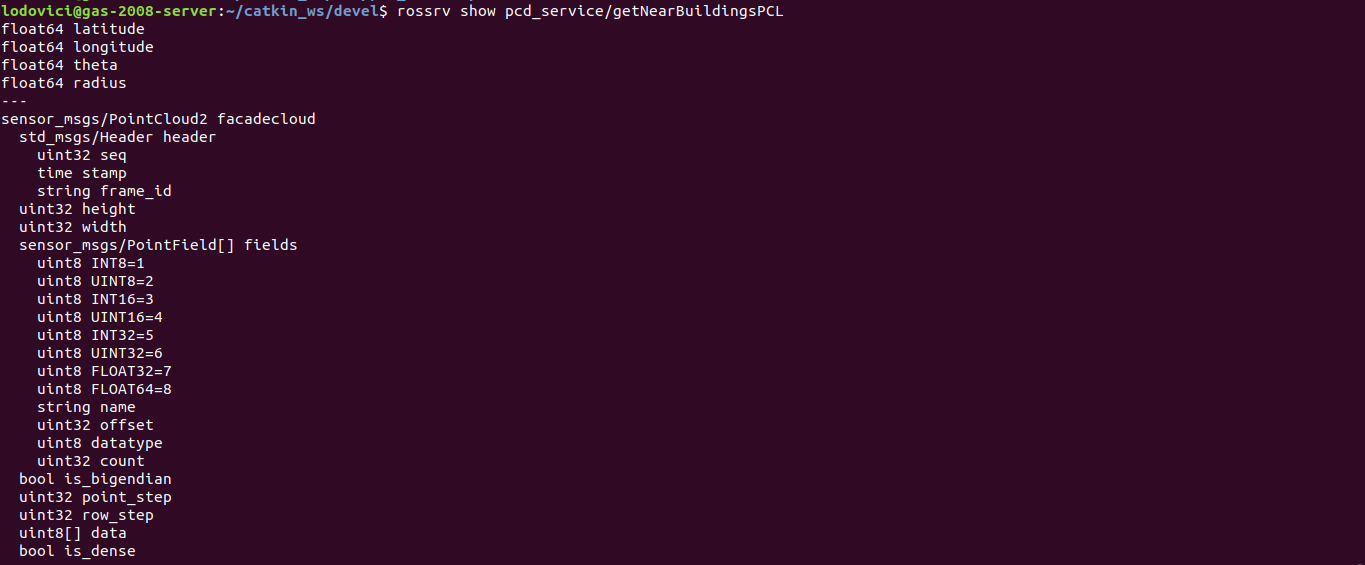
\includegraphics[width=0.9\textwidth]{Immagini/strutturamessaggio.png}
    \caption{Struttura del servizio di richiesta delle point cloud}
    \label{fig:QueryResult}
\end{figure}

Il servizio è stato poi testato facendo delle richieste grazie a \textit{rosservice call} che permette di interrogare i servizi ros
\begin{figure}[H]
    \centering
    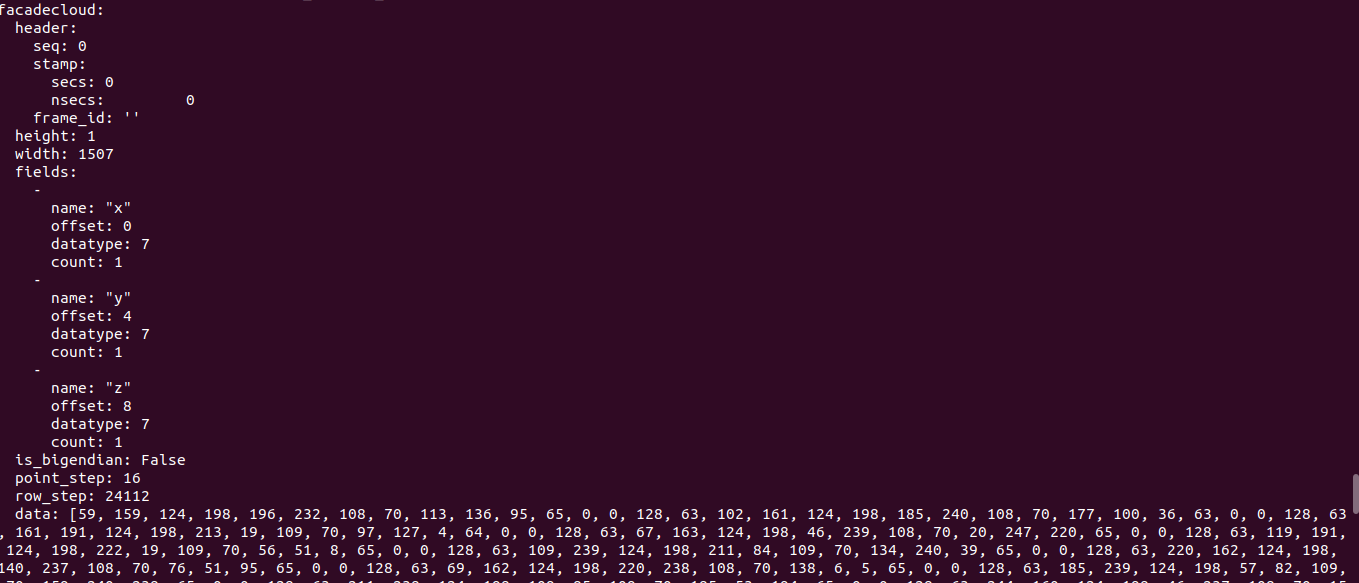
\includegraphics[width=0.9\textwidth]{Immagini/RispostaAlServizio.png}
    \caption{Si può notare che il servizio risponde con una pointcloud contenente la facciata dell'edificio corrente}
    \label{fig:QueryResult}
\end{figure}